\documentclass[english,ruled]{article}
\usepackage[T1]{fontenc}
\usepackage[latin9]{inputenc}
\usepackage{amsmath}
\usepackage{amssymb}
\usepackage{xcolor}
\usepackage{pgfplots}
\pgfplotsset{compat=1.15}
\usepackage[colorlinks]{hyperref}

\begin{document}

	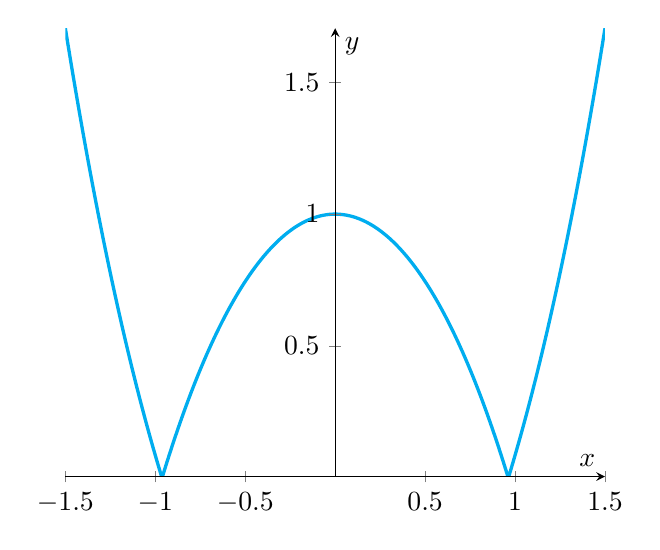
\begin{tikzpicture}
    \begin{axis}[
            axis on top,
            legend pos=outer north east,
            axis lines = center,
            xlabel = $x$,
            ylabel = $y$,
        ]
        \addplot[very thick,cyan,samples=500,domain=-1.5:1.5] {abs(e^x + e^(-x) - 3)};
    \end{axis}
\end{tikzpicture}

\end{document}